% 幺正性、支割线与 Cutkosky 关系
圈图中的内部传播子通常不在质量壳上，因此它们只是积分变量，并不对应可直接探测的中间粒子。随着外部总能量升高，某些内部线可能第一次同时满足正能质量壳条件；从这一阈值开始，积分中出现与真实中间态相同的相空间。Feynman 分母中的 $+\ii0^+$ 规定决定这个新贡献以怎样的虚部进入振幅。把“哪些内部线同时在壳”画成切开图以后，才得到通常所说的 Cutkosky 规则；所谓极点夹逼（pinch）只是这一阈值在复积分平面上的解析表现。


二体阈值的解析结构已经包含在两个标量传播子的共同分母中，与具体顶角分子无关。取完成 $k^0$ 轮廓积分后的标量泡图核
\begin{equation}
 \mathcal B(P^0)
 \equiv
 \int\frac{\dd^3 \mathbf k}{(2\pi\hbar)^3}
 \frac{c^2}{4E_1E_2}
 \left[
 \frac{1}{P^0c-E_1-E_2+\ii0^+}
 -\frac{1}{P^0c+E_1+E_2-\ii0^+}
 \right],
 \label{eq:qft-bubble-after-k0-dp8}
\end{equation}
其中
\begin{equation*}
 E_1=\sqrt{m_1^2c^4+c^2\mathbf k^2},
 \qquad
 E_2=\sqrt{m_2^2c^4+c^2(\mathbf P-\mathbf k)^2}.
\end{equation*}
对正的 $P^0$，只有第一项的分母能够在实积分域取零，因此其虚部为
\begin{align}
 \operatorname{Im}\mathcal B(P^0)
 &=-\pi
 \int\frac{\dd^3 \mathbf k}{(2\pi\hbar)^3}
 \frac{c^2}{4E_1E_2}
 \delta(P^0c-E_1-E_2).
 \label{eq:bubble-imag-phase-space-dp8}
\end{align}
这个 $\delta$ 函数正是“两个内部粒子同时成为真实正能粒子”的能量守恒条件。对等质量情形 $m_1=m_2=m$，质心系中的在壳动量和速度因子为
\begin{align}
 k_*^2
 &=\frac{s-4m^2c^2}{4},\\
 \beta_*(s)
 &\equiv\frac{ck_*}{E_{\rm cm}/2}
 =\sqrt{1-\frac{4m^2c^2}{s}}.
 \label{eq:two-body-threshold-beta-dp8}
\end{align}
因此二粒子连续谱只能在 $s\ge4m^2c^2$ 后打开，并在阈值附近按 $\beta_*(s)$ 从零增长。

传播子割线的局部规则来自同一个分布恒等式。先写单个 Feynman 分母跨过实轴的差：
\begin{equation}
 \operatorname{Disc}\frac1{q^2-m^2c^2+\ii0^+}
 =-2\pi\ii\,\delta(q^2-m^2c^2).
 \label{eq:feynman-denominator-discontinuity-dp68}
\end{equation}
物理中间态还必须选取正能支撑，于是图中被切开的标量传播子采用
\begin{equation}
 \boxed{
 \frac1{q^2-m^2c^2+\ii0^+}
 \quad\longrightarrow\quad
 -2\pi\ii\,\delta_+(q^2-m^2c^2)}
 \label{eq:cutkosky-propagator-rule-dp8}
\end{equation}
其中 $\delta_+(q^2-m^2c^2)\equiv\Theta(q^0)\delta(q^2-m^2c^2)$。若采用带显式 $\ii$ 的传播子定义，相应整体 $\ii$ 因子也必须按同一约定保留。

另一方面，前文散射幺正性正文\eqnrefs{eq:optical-unitarity-r68} 可以按耦合阶数逐阶展开。最低非平凡阶给出
\begin{equation}
 \boxed{
 2\operatorname{Im}\langle i|\hat T^{(2)}|i\rangle
 =\sum_X
 \langle i|\hat T^{(1)\dagger}|X\rangle
 \langle X|\hat T^{(1)}|i\rangle,}
 \label{eq:perturbative-optical-theorem-dp68}
\end{equation}
其中 $|X\rangle$ 是完整的真实在壳中间态。\eqnrefs{eq:cutkosky-propagator-rule-dp8} 正是把这一算符关系翻译成圈积分的逐图计算规则。

\begin{figure}[htbp]
 \centering
 
\includegraphics[width=0.78\textwidth]{two_body_cut_threshold.png}
 \caption{等质量二粒子割线的无量纲阈值因子 $\beta_*(s)$，由\eqnrefs{eq:two-body-threshold-beta-dp8} 直接计算。横轴 $x=\sqrt{s}/(2mc)$；$x=1$ 是二粒子阈值。该图只展示相空间开启因子，具体圈图的整体前因子和分子结构由相互作用决定。}
 \label{fig:two-body-cut-threshold-dp8}
\end{figure}

\begin{figure}[htbp]
 \centering
 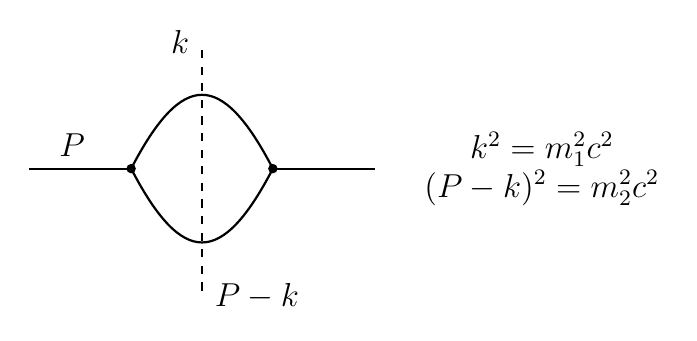
\begin{tikzpicture}[x=1cm,y=1cm,every node/.style={font=\large}]
 \coordinate (L) at (-2.2,0); \coordinate (R) at (2.2,0);
 \coordinate (a) at (-0.9,0); \coordinate (b) at (0.9,0);
 \draw[line width=.8pt] (L)--(a);
 \draw[line width=.8pt] (b)--(R);
 \draw[line width=.8pt] (a) .. controls (-0.25,1.25) and (0.25,1.25) .. (b);
 \draw[line width=.8pt] (a) .. controls (-0.25,-1.25) and (0.25,-1.25) .. (b);
 \fill (a) circle (1.7pt); \fill (b) circle (1.7pt);
 \draw[dashed,line width=1pt] (0,-1.55)--(0,1.55);
 \node at (-1.65,.3) {$P$};
 \node[anchor=south east,fill=white,inner sep=1pt] at (-.12,1.42) {$k$};
 \node[anchor=north west,fill=white,inner sep=1pt] at (.12,-1.42) {$P-k$};
 \node[align=center,right] at (2.7,0) {$k^2=m_1^2c^2$\\$(P-k)^2=m_2^2c^2$};
\end{tikzpicture}

 \caption{二体泡图的幺正性割线。虚线表示把两条内部传播子同时置于正能质量壳；割线积分使用的测度就是相应真实二体 Lorentz 不变相空间。}
 \label{fig:qft-bubble-cut-dp8}
\end{figure}
